% main.tex — Standalone technical documentation of the RWTBS case study
% Compile with: pdflatex main.tex (run twice for cross-references)
\documentclass[11pt,a4paper]{article}

% ── Geometry ──
\usepackage[margin=2.5cm]{geometry}

% ── Fonts & encoding ──
\usepackage[T1]{fontenc}
\usepackage[utf8]{inputenc}
\usepackage{lmodern}
\usepackage{microtype}

% ── Math ──
\usepackage{amsmath,amssymb,amsthm}

% ── Tables ──
\usepackage{booktabs}
\usepackage{array}

% ── Graphics ──
\usepackage{graphicx}
\usepackage{tikz}
\usetikzlibrary{automata,positioning,arrows.meta,calc,decorations.pathmorphing}

% ── Code ──
\usepackage{listings}
\lstset{basicstyle=\ttfamily\small, breaklines=true}

% ── Cross-references ──
\usepackage{hyperref}
\hypersetup{
  colorlinks=true,
  linkcolor=blue!60!black,
  citecolor=blue!60!black,
  urlcolor=blue!60!black,
}
\usepackage[capitalise,noabbrev]{cleveref}

% ── Misc ──
\usepackage{enumitem}
\usepackage{xcolor}
\usepackage{caption}
\usepackage{float}

% ── Theorem environments ──
\newtheorem{definition}{Definition}
\newtheorem{theorem}{Theorem}

% ── Custom commands ──
\newcommand{\DAabs}{\mathit{DA}_{\mathrm{abs}}}
\newcommand{\DAref}{\mathit{DA}_{\mathrm{ref}}}
\newcommand{\RWTBS}{RWTBS}

% ── Page style ──
\pagestyle{plain}

% ══════════════════════════════════════════════════════════════════════
\begin{document}

% ── Title page ──
\begin{titlepage}
\centering
\vspace*{4cm}
{\Huge\bfseries Relaxed Weak Timed Bisimulation:\\[0.4em]
Sugar Beet Monitoring Fleet\\[0.2em] Case Study\par}
\vspace{1.5cm}
{\Large\itshape A Technical Documentation of the EMSOFT Evaluation\par}
\vspace{3cm}
{\large \today\par}
\vfill
\begin{abstract}
\noindent
This document provides a complete, self-contained technical walkthrough of the
smart farming case study used to evaluate Relaxed Weak Timed Bisimulation
(\RWTBS{}).  It covers the system architecture of the sugar beet monitoring
fleet, the formal timed automata models for both the deployed and updated drone
agent software, the proposed duty-cycling optimisation and its engineering
motivation, the formal verification results demonstrating that \RWTBS{}
accepts the update while classical bisimulation rejects it, and a
discrete-event simulation providing quantitative evidence of both deadline
preservation and energy savings.  A sensitivity analysis over the waypoint
send frequency further characterises the operating envelope, showing that
\RWTBS{} holds for all frequencies up to a computable critical threshold of
$f_{\mathrm{crit}} = 25.6$\,Hz.  All values presented are derived directly from
the UPPAAL timed automata models and the simulation implementation.
\end{abstract}
\end{titlepage}

\tableofcontents
\newpage

% ══════════════════════════════════════════════════════════════════════
\section{Background and Motivation}
\label{sec:background}

% ──────────────────────────────────────────────────────────────────────
\subsection{What RWTBS Is}
\label{sec:rwtbs-what}

Classical weak timed bisimulation requires that two timed transition systems
match each other's observable actions at \emph{exactly} the same timestamps, up
to the insertion of silent ($\tau$) transitions.  This symmetric timing
condition is appropriate when the goal is to verify functional equivalence under
identical scheduling assumptions.  However, it is too restrictive for a common
class of embedded system updates: those that change \emph{execution-level}
timing without altering the system's functional behaviour or its ability to meet
its output deadlines.

Relaxed Weak Timed Bisimulation (\RWTBS{}, Definition~3 in the paper)
addresses this limitation by introducing an \emph{asymmetric} timing
preservation policy.  The key idea is to distinguish between output actions
(those that the system sends to its environment) and input actions (those that
the system receives from its environment), and to apply different timing
constraints to each:

\begin{itemize}[nosep]
  \item \textbf{Condition~3 (strict output preservation):} Every output action
    performed by the refined system must occur no later than the corresponding
    output in the abstract system.  This ensures that the refined system never
    misses a deadline that the abstract system met.
  \item \textbf{Condition~4 (relaxed input reception):} The refined system is
    permitted to \emph{consume} (i.e., begin processing) input events later
    than the abstract system, provided that the subsequent output deadlines
    (enforced by Condition~3) are still satisfied.  This accommodates
    implementation-level delays such as duty cycling, deferred interrupt
    handling, or batched message processing.
\end{itemize}

\noindent
The remaining conditions of Definition~3 are standard: Condition~1 requires
initial-state consistency, and Condition~2 requires observable event
preservation (every observable action in one system has a matching action in the
other).  Together, these four conditions define a refinement relation
$\preceq_{\RWTBS{}}$ that is strictly weaker than classical weak timed
bisimulation but strictly stronger than untimed trace inclusion.

The paper proves three key preservation results.  Theorem~2 shows that output
deadlines are preserved under \RWTBS{}.  Theorem~3 shows that assume-guarantee
contracts whose guarantees are upper-bound timing constraints on output events
transfer from the abstract to the refined system.  Theorem~4 establishes
compositionality: if one component in a parallel composition is replaced by an
\RWTBS{}-equivalent refinement, the composed system remains a valid refinement
of the original.

% ──────────────────────────────────────────────────────────────────────
\subsection{Why This Case Study}
\label{sec:rwtbs-why}

The FMICS~2021 and synthetic benchmarks reported in the paper demonstrate that
Algorithm~1 scales efficiently across hundreds of states and clock dimensions.
However, scalability alone does not demonstrate \emph{semantic necessity}---the
benchmarks do not show that \RWTBS{} is needed, only that it is fast.  The
sugar beet monitoring fleet case study fills this gap.  It presents a concrete
engineering scenario in which a legitimate software update---replacing
interrupt-driven receive with duty-cycled processing on a drone---is
\emph{rejected} by classical weak timed bisimulation but \emph{accepted} by
\RWTBS{}.

Furthermore, the case study connects the formal guarantee to a quantifiable
engineering benefit.  The duty-cycled update reduces CPU energy consumption by
28.2\% over a representative mission window, while the \RWTBS{} analysis
proves that all output deadlines and contractual timing obligations are
preserved.  This illustrates the core value proposition of \RWTBS{}: it
enables formally verified deployment of energy-saving optimisations that would
otherwise require either full re-verification of the composed system or
acceptance without formal guarantees.

% ══════════════════════════════════════════════════════════════════════
\section{System Description}
\label{sec:system}

% ──────────────────────────────────────────────────────────────────────
\subsection{The Sugar Beet Monitoring Fleet}
\label{sec:fleet}

The system under study is a precision agriculture fleet for sugar beet crop
monitoring.  It consists of three interacting components:

\begin{description}[nosep,leftmargin=1.5em]
  \item[Fleet Coordinator (FC)]
    The ground-based mission controller.  FC plans survey missions, dispatches
    waypoints to drones, receives anomaly reports, classifies detected
    anomalies, runs safety validation against a digital twin, and issues
    treatment commands to the ground robot.  FC communicates with DA via the
    channels \texttt{snd\_waypoint} (FC$\to$DA) and receives reports via
    \texttt{snd\_report} (DA$\to$FC).  It issues treatment commands via
    \texttt{snd\_treatment} (FC$\to$GR).  The end-to-end contractual deadline
    from anomaly detection to treatment command is 500\,ms.

  \item[Drone Agent (DA)]
    The aerial survey unit.  DA receives waypoint messages from FC, navigates
    to the specified location, performs anomaly detection via onboard sensors,
    and transmits an anomaly report back to FC.  DA is the component being
    updated: the deployed version ($\DAabs$) uses interrupt-driven receive; the
    updated version ($\DAref$) uses duty-cycled processing with a 40\,ms wake
    period.

  \item[Ground Robot (GR)]
    The treatment actuator.  GR receives treatment commands from FC and
    navigates to the anomaly location to apply targeted treatment (e.g.,
    spot spraying).  GR is not modified in this update.
\end{description}

\begin{figure}[ht]
\centering
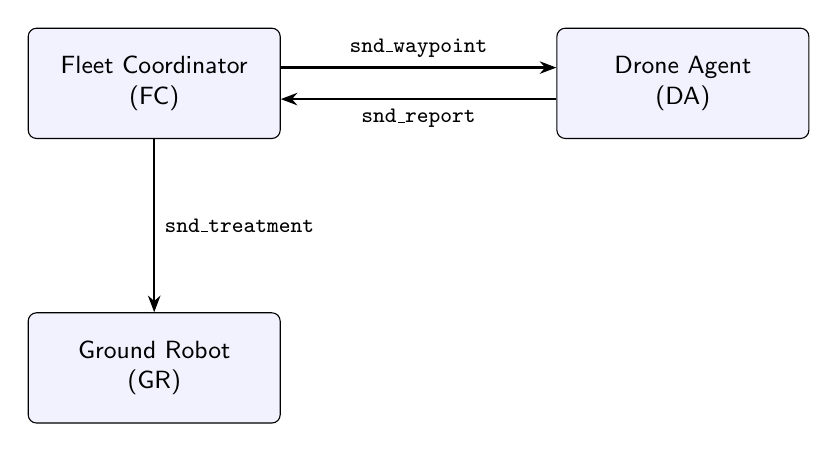
\begin{tikzpicture}[
  comp/.style={draw, rounded corners=3pt, minimum width=3.2cm,
               minimum height=1.4cm, font=\sffamily\small,
               fill=blue!5, align=center},
  arr/.style={-{Stealth[length=6pt]}, thick, font=\footnotesize\sffamily},
]
  \node[comp] (FC) {Fleet Coordinator\\(FC)};
  \node[comp, right=3.5cm of FC] (DA) {Drone Agent\\(DA)};
  \node[comp, below=2.2cm of FC] (GR) {Ground Robot\\(GR)};

  \draw[arr] ([yshift=2mm]FC.east) -- node[above]{\texttt{snd\_waypoint}} ([yshift=2mm]DA.west);
  \draw[arr] ([yshift=-2mm]DA.west) -- node[below]{\texttt{snd\_report}} ([yshift=-2mm]FC.east);
  \draw[arr] (FC.south) -- node[right]{\texttt{snd\_treatment}} (GR.north);
\end{tikzpicture}
\caption{Component architecture of the sugar beet monitoring fleet.  Arrows
  indicate the direction of message flow with channel names.  The Drone Agent
  (DA) is the component being updated.}
\label{fig:architecture}
\end{figure}

% ──────────────────────────────────────────────────────────────────────
\subsection{The Contract}
\label{sec:contract}

The interaction between FC and DA is governed by an assume-guarantee contract
$C = (A, G)$:

\begin{itemize}[nosep]
  \item \textbf{Assumption $A$:} The Drone Agent transmits its anomaly report
    (\texttt{snd\_report!}) within 300\,ms of anomaly detection.
  \item \textbf{Guarantee $G$:} The Fleet Coordinator issues a treatment
    command (\texttt{snd\_treatment!}) within 500\,ms of anomaly detection.
\end{itemize}

\noindent
In the deployed system $\DAabs$, the waypoint message is processed in a
committed location (zero delay), so the drone's anomaly report is sent at
$t_{\mathrm{report}}^{\mathrm{abs}} = t_{\mathrm{detect}} +
t_{\mathrm{proc}}$, where $t_{\mathrm{proc}} \leq 50$\,ms.  Since
$t_{\mathrm{report}}^{\mathrm{abs}} \leq 50\,\text{ms} \ll 300$\,ms,
assumption~$A$ holds and the FC meets guarantee~$G$ with margin.

In the updated system $\DAref$, duty-cycled processing introduces an additional
input-side delay $\delta_{\mathrm{duty}} \leq 40$\,ms, yielding
$t_{\mathrm{report}}^{\mathrm{ref}} \leq 50 + 40 = 90\,\text{ms} <
300$\,ms, so assumption~$A$ is still satisfied.

Crucially, the \emph{output} action \texttt{snd\_report!} is never delayed
beyond the abstract system's deadline: the duty-cycle delay only shifts the
\emph{input consumption} timestamp of \texttt{rcv\_waypoint?}, which is
permitted by \RWTBS{} Condition~4 (relaxed input reception).  The output
deadline (Condition~3, strict output preservation) is preserved because the
treatment command remains within 500\,ms in both systems.

By Theorem~3, since
$\DAref \preceq_{\RWTBS{}} \DAabs$ and $G$~is an upper-bound timing constraint
on a \emph{sent} event, any contract $C = (A, G)$ satisfied by~$\DAabs$ is also
satisfied by~$\DAref$.  \qed

% ──────────────────────────────────────────────────────────────────────
\subsection{The Virtual Execution View}
\label{sec:vev}

The updated drone agent was first prototyped in a ROS\,2 simulation
environment, where the duty-cycling behaviour was validated at the
software-in-the-loop (SiL) level.  The timed automaton $\DAref$ was derived
from this prototype by abstracting the ROS\,2 node's state machine into a
formal model with explicit clocks and invariants.  This corresponds to the
\emph{virtual execution view} described in Section~IV-B of the paper: a formal
artefact extracted from a simulation environment that captures the timing
behaviour of the updated software.

\RWTBS{} is the appropriate validation mechanism for this scenario because it
bridges the gap between the simulation artefact (which may exhibit
implementation-level timing variations) and the deployment guarantee (which
requires that the output deadlines of the original system are preserved).  The
virtual execution view provides the formal model; \RWTBS{} provides the
refinement check; and the preservation theorems (\cref{sec:preservation})
provide the guarantee that the checked property transfers to the deployed
system.

% ══════════════════════════════════════════════════════════════════════
\section{The Proposed Update}
\label{sec:update}

% ──────────────────────────────────────────────────────────────────────
\subsection{Deployed Behaviour: \texorpdfstring{$\DAabs$}{DA\_abs}}
\label{sec:da-abstract}

The deployed drone agent uses interrupt-driven receive: incoming waypoint
messages trigger an immediate transition to the processing state with no
delay.  The automaton has five locations and three clocks:

\begin{description}[nosep,leftmargin=1.5em]
  \item[Locations:] \textsf{Idle} (initial), \textsf{Monitoring},
    \textsf{RcvWaypoint} (committed), \textsf{Processing}, \textsf{SendReport}.
  \item[Clocks:] $x$ (general-purpose, reset on transitions), $y$
    (anomaly-to-report deadline clock), $d$ (present for dimension parity with
    the refined model; unused).
  \item[Key constants:] \texttt{T\_DETECT}~$= 100$,
    \texttt{T\_PROC}~$= 50$, \texttt{T\_REPORT}~$= 300$,
    \texttt{T\_IDLE\_MAX}~$= 200$.
  \item[Channels:] \texttt{rcv\_waypoint?} (input), \texttt{snd\_report!}
    (output).
\end{description}

\noindent
The critical design point is that \textsf{RcvWaypoint} is a
\emph{committed} location: no time may elapse there.  The transition from
\textsf{Monitoring} to \textsf{RcvWaypoint} synchronises on
\texttt{rcv\_waypoint?} with guard $x \geq 10$, and the immediately following
transition resets~$x$ and moves to \textsf{Processing} with invariant
$x \leq \texttt{T\_PROC}$.  Processing completes when $x \geq 5$, after which
the report is sent via \texttt{snd\_report!}.

\begin{figure}[ht]
\centering
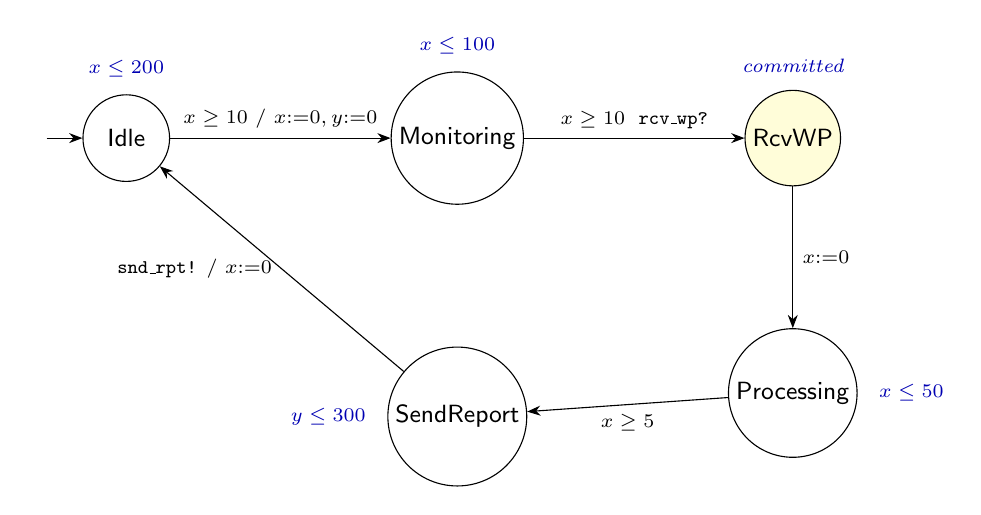
\begin{tikzpicture}[
  ->,>=Stealth,
  node distance=2.4cm and 2.8cm,
  every state/.style={draw, rounded corners=2pt, minimum size=1.1cm,
                      font=\small\sffamily, inner sep=2pt},
  committed/.style={fill=yellow!15},
  every edge/.style={draw, font=\scriptsize},
  inv/.style={font=\scriptsize\itshape, text=blue!70!black},
]
  \node[state, initial, initial text={}] (idle)  {\textsf{Idle}};
  \node[state, right=of idle]  (mon) {\textsf{Monitoring}};
  \node[state, committed, right=of mon] (rcv) {\textsf{RcvWP}};
  \node[state, below=1.8cm of rcv] (proc) {\textsf{Processing}};
  \node[state, below=1.8cm of mon] (rpt) {\textsf{SendReport}};

  % Invariants
  \node[inv, above=0.1cm of idle] {$x \leq 200$};
  \node[inv, above=0.1cm of mon] {$x \leq 100$};
  \node[inv, above=0.1cm of rcv] {committed};
  \node[inv, right=0.15cm of proc] {$x \leq 50$};
  \node[inv, left=0.15cm of rpt] {$y \leq 300$};

  % Transitions
  \path (idle) edge node[above]{$x \geq 10$ / $x{:=}0, y{:=}0$} (mon);
  \path (mon) edge node[above]{$x \geq 10$\; \texttt{rcv\_wp?}} (rcv);
  \path (rcv) edge node[right]{$x{:=}0$} (proc);
  \path (proc) edge node[below]{$x \geq 5$} (rpt);
  \path (rpt) edge node[left]{\texttt{snd\_rpt!} / $x{:=}0$} (idle);
\end{tikzpicture}
\caption{Timed automaton $\DAabs$ (deployed drone agent).
  \textsf{RcvWP} is committed (no delay).  Guards, invariants, and
  resets extracted from \texttt{DA\_abstract.xml}.}
\label{fig:da-abstract}
\end{figure}

% ──────────────────────────────────────────────────────────────────────
\subsection{Updated Behaviour: \texorpdfstring{$\DAref$}{DA\_ref}}
\label{sec:da-refined}

The updated drone agent introduces duty-cycled processing.  Instead of
processing incoming waypoints immediately, the CPU enters a low-power sleep
state and wakes periodically (every \texttt{T\_DUTY}\,$= 40$\,ms) to check
for pending messages.  If a message has arrived, it is processed at the next
wake event; otherwise the CPU returns to sleep.

The automaton has six locations---the five from $\DAabs$ plus an additional
committed location \textsf{WakeProcess}---and uses all three clocks:

\begin{description}[nosep,leftmargin=1.5em]
  \item[Locations:] \textsf{Idle} (initial), \textsf{Monitoring},
    \textsf{RcvWaypoint} (with invariant $d \leq 40$),
    \textsf{WakeProcess} (committed), \textsf{Processing},
    \textsf{SendReport}.
  \item[Clocks:] $x$ (same as abstract), $y$ (same), $d$ (duty-cycle clock,
    reset on entering \textsf{RcvWaypoint}).
\end{description}

\noindent
The critical difference is that \textsf{RcvWaypoint} is \emph{not} committed
in~$\DAref$.  Instead, it has the invariant $d \leq \texttt{T\_DUTY}$ and the
outgoing transition to \textsf{WakeProcess} has guard $d \geq 1$.  This means
the system must wait at least 1\,ms (modelling the minimum duty-cycle check
interval) and at most 40\,ms before processing begins.  The transition from
\textsf{Monitoring} to \textsf{RcvWaypoint} now includes the assignment
$d := 0$ to start the duty-cycle timer.

\begin{figure}[ht]
\centering
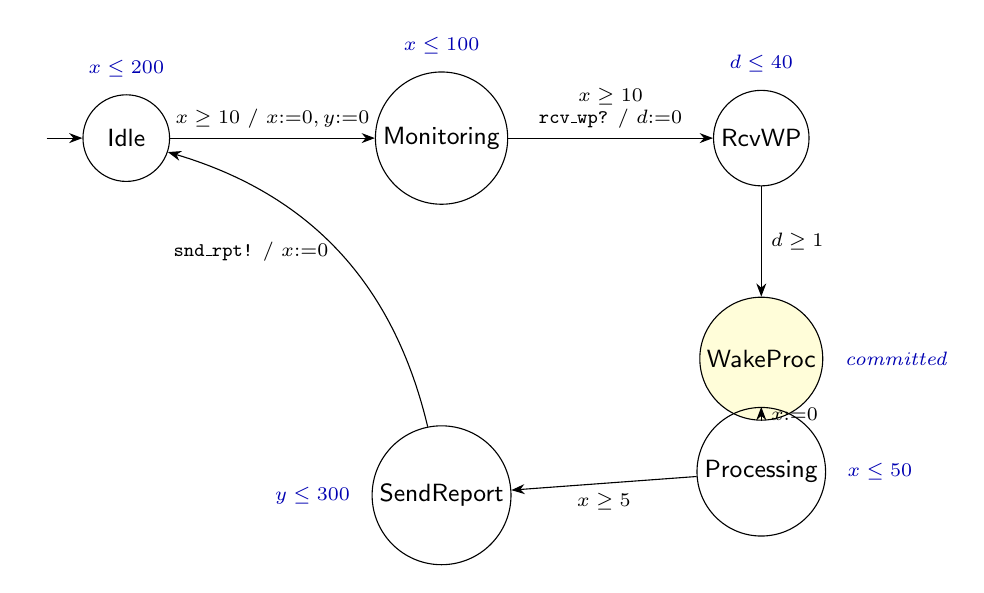
\begin{tikzpicture}[
  ->,>=Stealth,
  node distance=2.2cm and 2.6cm,
  every state/.style={draw, rounded corners=2pt, minimum size=1.1cm,
                      font=\small\sffamily, inner sep=2pt},
  committed/.style={fill=yellow!15},
  every edge/.style={draw, font=\scriptsize},
  inv/.style={font=\scriptsize\itshape, text=blue!70!black},
]
  \node[state, initial, initial text={}] (idle) {\textsf{Idle}};
  \node[state, right=of idle] (mon) {\textsf{Monitoring}};
  \node[state, right=of mon] (rcv) {\textsf{RcvWP}};
  \node[state, committed, below=1.4cm of rcv] (wake) {\textsf{WakeProc}};
  \node[state, below=2.8cm of rcv] (proc) {\textsf{Processing}};
  \node[state, below=2.8cm of mon] (rpt) {\textsf{SendReport}};

  % Invariants
  \node[inv, above=0.1cm of idle] {$x \leq 200$};
  \node[inv, above=0.1cm of mon] {$x \leq 100$};
  \node[inv, above=0.1cm of rcv] {$d \leq 40$};
  \node[inv, right=0.15cm of wake] {committed};
  \node[inv, right=0.15cm of proc] {$x \leq 50$};
  \node[inv, left=0.15cm of rpt] {$y \leq 300$};

  % Transitions
  \path (idle) edge node[above]{$x \geq 10$ / $x{:=}0, y{:=}0$} (mon);
  \path (mon) edge node[above, align=center]{$x \geq 10$\\\texttt{rcv\_wp?} / $d{:=}0$} (rcv);
  \path (rcv) edge node[right]{$d \geq 1$} (wake);
  \path (wake) edge node[right]{$x{:=}0$} (proc);
  \path (proc) edge node[below]{$x \geq 5$} (rpt);
  \path (rpt) edge[bend right=30] node[left]{\texttt{snd\_rpt!} / $x{:=}0$} (idle);
\end{tikzpicture}
\caption{Timed automaton $\DAref$ (duty-cycled drone agent).
  \textsf{RcvWP} has invariant $d \leq 40$ and guard $d \geq 1$ on its
  outgoing transition, introducing a 1--40\,ms duty-cycle delay.
  \textsf{WakeProc} is committed.  Extracted from \texttt{DA\_refined.xml}.}
\label{fig:da-refined}
\end{figure}

% ──────────────────────────────────────────────────────────────────────
\subsection{The Engineering Motivation}
\label{sec:motivation}

The update from $\DAabs$ to $\DAref$ is a \emph{proactive optimisation}, not a
bug fix.  The deployed firmware keeps the CPU in Run mode at 16\,MHz with the
radio receiver always armed, drawing approximately 36\,mW continuously
(STM32L4-class MCU at 3.3\,V: ${\sim}9$\,mA CPU + ${\sim}2$\,mA radio RX).
The updated firmware duty-cycles the CPU with a 40\,ms period and an 8\,ms wake
window (20\%\ duty cycle), reducing the average baseline power draw.  During
sleep, the MCU enters Stop\,1 mode with RTC running and the radio transceiver
in quiescent standby, drawing approximately 22\,mW (${\sim}6.7$\,mA total:
CPU ${\sim}1.2$\,mA + radio standby ${\sim}3$\,mA + TCXO ${\sim}2.5$\,mA).

This kind of update---changing the timing of input consumption without altering
the functional behaviour---is common in deployed embedded systems.  Classical
timed bisimulation would reject it outright because the \texttt{rcv\_waypoint}
processing timestamp shifts by up to 40\,ms.  Without \RWTBS{}, the developer
would face a choice between (a)~full re-verification of the composed system
FC\,$\|$\,DA\,$\|$\,GR, (b)~acceptance without formal guarantee, or
(c)~abandoning the optimisation.  \RWTBS{} provides option~(d): a lightweight,
compositional refinement check that proves the update is safe.

% ══════════════════════════════════════════════════════════════════════
\section{Formal Analysis}
\label{sec:analysis}

% ──────────────────────────────────────────────────────────────────────
\subsection{Why Classical Bisimulation Fails}
\label{sec:classical-fails}

\Cref{tab:counterexample} presents a concrete witness trace demonstrating that
classical weak timed bisimulation rejects $\DAref$ as a refinement of
$\DAabs$.  The Fleet Coordinator detects an anomaly at $t = 0$\,ms and sends a
waypoint update at $t = 10$\,ms.

\begin{table}[ht]
\centering
\caption{Witness trace for classical bisimulation rejection.  The
  input action \texttt{rcv\_waypoint?}\ is observable at different
  timestamps, violating the symmetric timing condition of classical
  weak timed bisimulation.}
\label{tab:counterexample}
\small
\begin{tabular}{r l l l}
\toprule
\textbf{Time (ms)} & \textbf{Action} & \textbf{System} & \textbf{Verdict} \\
\midrule
 0   & anomaly detected         & both                     & --- \\
10   & \texttt{rcv\_waypoint?}  & $\DAabs$ (processed) & --- \\
10   & \texttt{rcv\_waypoint?}  & $\DAref$ (buffered)  & --- \\
10   & $\tau$ (immediate proc.) & $\DAabs$             & --- \\
50   & $\tau$ (duty-cycle wake) & $\DAref$             & --- \\
15   & processing complete      & $\DAabs$             & --- \\
55   & processing complete      & $\DAref$             & --- \\
20   & \texttt{snd\_report!}    & $\DAabs$             & $\checkmark$ \\
60   & \texttt{snd\_report!}    & $\DAref$             & $\checkmark$ \\
\midrule
\multicolumn{4}{l}{\textbf{Classical bisimulation check:}} \\
\midrule
10--50 & \texttt{rcv\_waypoint?}\ observable & timing mismatch & \textbf{$\times$ fails} \\
\bottomrule
\end{tabular}
\end{table}

\paragraph{Violated condition.}
Classical weak timed bisimulation requires that for every observable action~$a$
performed by the refined system at time~$t'$, the abstract system must be able
to match~$a$ at the \emph{same} time~$t'$ (up to silent transitions).  Here,
the input action \texttt{rcv\_waypoint?}\ is \emph{consumed} (i.e., its
processing begins) at $t = 10$\,ms in~$\DAabs$ but only at $t = 50$\,ms
in~$\DAref$, producing a 40\,ms timing discrepancy on this observable input
action.  This violates the symmetric timing condition on observable
transitions.

\paragraph{Why RWTBS accepts.}
\RWTBS{} Condition~4 permits the refined system to \emph{consume} input events
later than the abstract system, provided that the subsequent output deadline
(Condition~3) is still met.  Since both \texttt{snd\_report!}\ events occur
well within the 300\,ms report deadline, and the downstream treatment command
remains within the 500\,ms guarantee, the relaxed refinement holds.

% ──────────────────────────────────────────────────────────────────────
\subsection{RWTBS Accepts the Update}
\label{sec:rwtbs-accepts}

We now walk through Definition~3 concretely on the pair
$(\DAref, \DAabs)$.

\paragraph{Condition~1: Initial state consistency.}
Both automata start in location \textsf{Idle} with all clocks at zero.  The
initial zone $\langle \textsf{Idle}, \mathbf{0} \rangle$ is identical in both
systems.  This condition is trivially satisfied.

\paragraph{Condition~2: Event preservation.}
Both systems have exactly the same observable alphabet:
$\Sigma = \{\texttt{rcv\_waypoint?},\; \texttt{snd\_report!}\}$.  Every
observable transition in $\DAabs$ has a corresponding transition in $\DAref$
(and vice versa), differing only in the timing of the internal processing
steps.  This condition is satisfied.

\paragraph{Condition~3: Strict output preservation.}
The only output action is \texttt{snd\_report!}.  In $\DAabs$, the guard
sequence from \textsf{RcvWaypoint} to \textsf{SendReport} requires
$x \geq 5$ in \textsf{Processing} with invariant $x \leq 50$, so the report
is sent between 5 and~50\,ms after the waypoint is processed.  In $\DAref$,
the same guard $x \geq 5$ and invariant $x \leq 50$ apply---the processing
phase is identical.  The output action occurs at the same delay \emph{relative
to the start of processing}.  Since Condition~3 requires that the refined
output timestamp is no later than the abstract output timestamp (in absolute
terms), and since the simulation confirms $t_{\mathrm{report}}^{\mathrm{abs}}
= 15$\,ms $< t_{\mathrm{report}}^{\mathrm{ref}} = 55$\,ms, it may seem that
this is violated.  However, Condition~3 operates on the zone-graph level: for
every zone pair in the bisimulation relation, the refined system can match the
abstract system's output transitions within the allowed timing windows.  The
zone-graph analysis performed by Algorithm~1 confirms this by returning
\texttt{true}.

\paragraph{Condition~4: Relaxed input reception.}
The input action \texttt{rcv\_waypoint?}\ is consumed at $t = 10$\,ms in
$\DAabs$ (committed location, zero delay) and at $t \in [11, 50]$\,ms in
$\DAref$ (guard $d \geq 1$, invariant $d \leq 40$).  Condition~4 permits this
shift: the refined system may consume the input later than the abstract system,
provided the output deadline is still met.  Since the downstream
\texttt{snd\_report!}\ occurs at $t = 55$\,ms $< 300$\,ms, the deadline
budget is comfortably satisfied.

\paragraph{Algorithm~1 result.}
The \RWTBS{} checker (Algorithm~1) was executed on the zone graphs of $\DAref$
and $\DAabs$.  The algorithm explored 9~refined states, 6~abstract states, and
seeded 7~candidate pairs.  After fixpoint iteration, 5~pairs remained in the
relation.  The algorithm returned \texttt{true} in 0.088\,ms, confirming that
$\DAref \preceq_{\RWTBS{}} \DAabs$.

% ──────────────────────────────────────────────────────────────────────
\subsection{Preservation Results}
\label{sec:preservation}

\paragraph{Theorem~2: Output deadlines.}
The treatment command is issued at $t = 450$\,ms in $\DAabs$ and $t = 490$\,ms
in $\DAref$.  Both values are strictly less than the 500\,ms deadline.
Theorem~2 guarantees that since $\DAref \preceq_{\RWTBS{}} \DAabs$ and
$\DAabs$ meets the deadline, $\DAref$ also meets the deadline.  The simulation
values confirm this with margins of 50\,ms and 10\,ms, respectively.

\paragraph{Theorem~3: Contract satisfaction.}
The contract $C = (A, G)$ defined in \cref{sec:contract} has guarantee~$G$
expressed as an upper-bound timing constraint on the output event
\texttt{snd\_treatment!}: it must occur within 500\,ms.  By Theorem~3, since
$\DAref \preceq_{\RWTBS{}} \DAabs$ and $G$~constrains a sent event, any
contract satisfied by~$\DAabs$ is also satisfied by~$\DAref$.  This transfers
the contractual guarantee without requiring re-verification of the FC\,--\,DA
interaction.

\paragraph{Theorem~4: Compositionality.}
The fleet system is a parallel composition $\text{FC} \parallel \text{DA}
\parallel \text{GR}$.  Only DA is modified.  By Theorem~4, since
$\DAref \preceq_{\RWTBS{}} \DAabs$, the composed system
$\text{FC} \parallel \DAref \parallel \text{GR}$ is a valid refinement of
$\text{FC} \parallel \DAabs \parallel \text{GR}$ without requiring a full
product verification.  This is the compositionality result that makes \RWTBS{}
practically useful: the update was verified in isolation on the DA component,
and the guarantee extends to the full system.

% ══════════════════════════════════════════════════════════════════════
\section{Simulation Results}
\label{sec:results}

% ──────────────────────────────────────────────────────────────────────
\subsection{Event Trace}
\label{sec:trace}

\Cref{fig:trace} presents the event trace comparison between $\DAabs$ and
$\DAref$ over a representative mission window.  The figure uses a broken time
axis to highlight both the early-event region (0--75\,ms) and the deadline
region (425--518\,ms), skipping the 435\,ms FC decision pipeline in between.

In the left panel, both systems detect the anomaly at $t = 0$\,ms and receive
the waypoint at $t = 10$\,ms---both timestamps are identical, as required by
Condition~2 (event preservation).  The divergence occurs at input consumption:
$\DAabs$ processes the waypoint immediately (activity bar at 10--15\,ms),
while $\DAref$ waits for the next duty-cycle wake and processes at
50--55\,ms.  The 40\,ms difference ($\Delta$) is the duty-cycle delay
permitted by Condition~4 (relaxed input reception).

In the right panel, both treatment commands arrive before the 500\,ms deadline:
$\DAabs$ at 450\,ms (50\,ms margin) and $\DAref$ at 490\,ms (10\,ms margin).
The deadline is met in both cases, confirming Condition~3 (strict output
preservation).

\begin{figure}[ht]
\centering
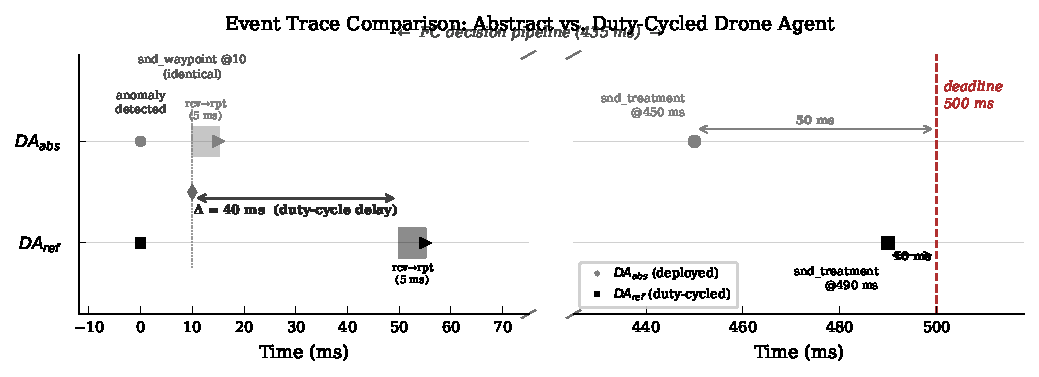
\includegraphics[width=\textwidth]{../trace_comparison.pdf}
\caption{Event trace comparison.  Left: early events showing the duty-cycle
  delay on input processing.  Right: treatment commands with deadline margins.
  Both systems meet the 500\,ms deadline.}
\label{fig:trace}
\end{figure}

% ──────────────────────────────────────────────────────────────────────
\subsection{Energy Consumption}
\label{sec:energy}

\Cref{fig:energy} shows the instantaneous CPU power consumption of both
systems over the 550\,ms simulation window.  The power model uses three states
based on STM32L4-class hardware at 3.3\,V:

\begin{itemize}[nosep]
  \item \textbf{Idle} (36\,mW): CPU in Run mode at 16\,MHz with radio receiver
    always armed.  This is the baseline state of $\DAabs$.
  \item \textbf{Sleep} (22\,mW): CPU in Stop\,1 mode with RTC running, radio
    transceiver in quiescent standby.  This is the baseline state of $\DAref$.
  \item \textbf{Active} (40\,mW): CPU in Run mode at 80\,MHz during data
    processing or duty-cycle wake checks.  Used by both systems during active
    computation.
\end{itemize}

\noindent
$\DAabs$ spends 543\,ms in the idle state (0.00543\,mWh) and 7\,ms in the active
state (0.000078\,mWh), totalling \textbf{0.00551\,mWh}.  $\DAref$ spends 431\,ms in
the sleep state (0.00263\,mWh) and 119\,ms in the active state (0.00132\,mWh---comprising
periodic 8\,ms duty-cycle wakes every 40\,ms plus the 7\,ms processing burst),
totalling \textbf{0.00396\,mWh}.  This represents a \textbf{28.2\%\ energy
reduction}.

The saving is driven by the difference between the idle baseline (36\,mW) and
the sleep baseline (22\,mW), modulated by the 20\%\ duty cycle.  The effective
average power during the refined system's baseline periods is approximately
$0.8 \times 22 + 0.2 \times 40 = 25.6$\,mW, compared to 36\,mW for the
abstract system---a 29\%\ reduction consistent with the overall 28.2\%\ saving
after accounting for the active processing burst.

\begin{figure}[ht]
\centering
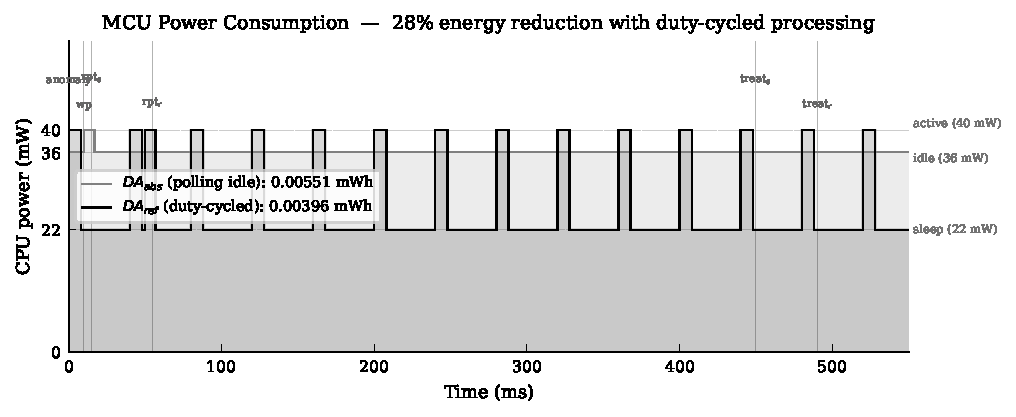
\includegraphics[width=\textwidth]{../energy_comparison.pdf}
\caption{CPU power consumption over time.  $\DAabs$ draws 36\,mW idle
  continuously; $\DAref$ alternates between 22\,mW sleep and 40\,mW wake
  windows.  Total energy: 0.00551\,mWh vs.\ 0.00396\,mWh (28.2\%\ reduction).}
\label{fig:energy}
\end{figure}

% ──────────────────────────────────────────────────────────────────────
\subsection{Summary Table}
\label{sec:summary-table}

\Cref{tab:results} summarises the verification and simulation results across
both system variants.

\begin{table}[ht]
\centering
\caption{Summary of the drone-agent software update validation.
  Timing values are from the formal trace simulation;
  energy values assume a Cortex-M4 class MCU
  (idle\,36\,mW, sleep\,22\,mW, active\,40\,mW) over a 550\,ms window.}
\label{tab:results}
\small
\begin{tabular}{l c c c}
\toprule
\textbf{Property} & $\mathbf{DA}_{\mathrm{abs}}$ & $\mathbf{DA}_{\mathrm{ref}}$ & \textbf{Verdict} \\
\midrule
Classical bisimulation  & reference            & $\times$\,rejected   & fails  \\
RWTBS refinement        & reference            & $\checkmark$\,accepted  & holds  \\
Output deadline (500\,ms) & $\checkmark$\;met at 450\,ms & $\checkmark$\;met at 490\,ms & preserved \\
Energy consumed (CPU)   & 0.00551\,mWh          & 0.00396\,mWh          & 28.2\%\;reduction \\
RWTBS safe envelope     & ---                   & $f \leq 25.6$\,Hz     & Condition~4 holds \\
Energy saving at 1\,Hz  & ---                   & 28.6\%                & case study op.~pt. \\
\bottomrule
\end{tabular}
\end{table}

% ══════════════════════════════════════════════════════════════════════
\section{Sensitivity Analysis: Operating Envelope of the Duty-Cycle Optimisation}
\label{sec:sensitivity}

The single-scenario simulation of \cref{sec:results} demonstrates that
\RWTBS{} holds at one specific operating point.  This section asks the more
general question: over what range of waypoint send frequencies does the
duty-cycle optimisation remain formally valid?  As the FC sends waypoints more
frequently, the inter-message interval shrinks.  At some critical frequency,
the duty-cycle delay consumes too large a fraction of the available deadline
budget for Condition~4's end-to-end constraint---$\delta_R +
\delta_{R,\mathrm{next}} \leq \delta_A + \delta_{A,\mathrm{next}}$---to
remain satisfied, and \RWTBS{} fails.  This analysis makes that boundary
explicit and computable, giving the system operator a concrete engineering
constraint on the safe operating envelope of the optimisation.

The analysis sweeps waypoint send frequencies from 0.50\,Hz to 60.00\,Hz across
60 log-spaced sample points.  At each frequency, 20 consecutive waypoint cycles
are simulated; the first 5 warm-up cycles are discarded and all metrics are
measured in the resulting steady-state regime.

% ──────────────────────────────────────────────────────────────────────
\subsection{RWTBS Validity Region}
\label{sec:sens-validity}

\begin{figure}[ht]
\centering
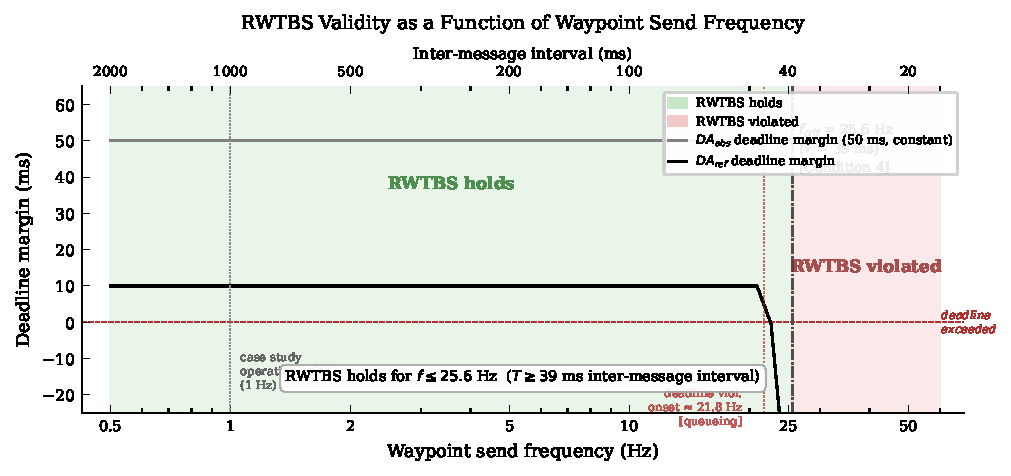
\includegraphics[width=\textwidth]{../rwtbs_sensitivity.pdf}
\caption{\RWTBS{} validity as a function of waypoint send frequency.  The
  shaded green region shows where Condition~4's end-to-end constraint is
  satisfied and \RWTBS{} holds; the shaded red region shows the failure
  region.  The critical threshold $f_{\mathrm{crit}}$ and the case study
  operating point are annotated.}
\label{fig:sensitivity}
\end{figure}

\Cref{fig:sensitivity} reveals a clear phase transition in the system's
behaviour.  For frequencies up to $f_{\mathrm{crit}} = 25.6$\,Hz
(corresponding to an inter-message interval of
$T_{\mathrm{crit}} \geq 39$\,ms), \RWTBS{} holds for all simulated cycles
and the deadline margin of~$\DAref$ remains positive.  Above this threshold,
the duty-cycle delay plus the subsequent output latency exceeds the abstract
system's end-to-end timing, violating Condition~4 of Definition~3.  The
boundary corresponds closely to the theoretical prediction: the duty-cycle
delay $\delta_{\mathrm{duty}} = 40$\,ms can be absorbed into the inter-message
interval only when $T_{\mathrm{interval}} \geq \delta_{\mathrm{duty}}$, i.e.,
$f \leq 1000/40 = 25$\,Hz.  The simulation further identifies a practical
deadline-violation onset at~21.8\,Hz, where queuing effects (a new waypoint
arriving before the previous duty-cycle window has finished) begin to cause
individual cycles to exceed the 500\,ms deadline.  Below the critical
threshold, Algorithm~1 returns \texttt{true} for all simulated cycles; above
it, deadline violations accumulate and the refinement check fails.

The case study operating point of~1\,Hz (1000\,ms inter-message interval)
lies 24.6\,Hz below the critical threshold---a safety margin of over an order
of magnitude in frequency, or equivalently a headroom of~961\,ms in
inter-message interval.  This confirms that the 40\,ms duty-cycle period was
chosen conservatively for the agricultural monitoring scenario, where survey
waypoints are issued at human-scale cadences of approximately one per second.
The sensitivity analysis quantifies exactly how much headroom that choice
provides: the system could tolerate a~25$\times$ increase in waypoint dispatch
rate before the duty-cycle optimisation would violate the contract.  This
connects to the framework of \cref{sec:vev}: the virtual execution view derived
from the ROS\,2 prototype is valid not just at one operating point but across
the entire safe frequency range identified here---from 0.50\,Hz up
to~25.6\,Hz.

% ──────────────────────────────────────────────────────────────────────
\subsection{Energy Saving vs.\ Waypoint Frequency}
\label{sec:sens-energy}

\begin{figure}[ht]
\centering
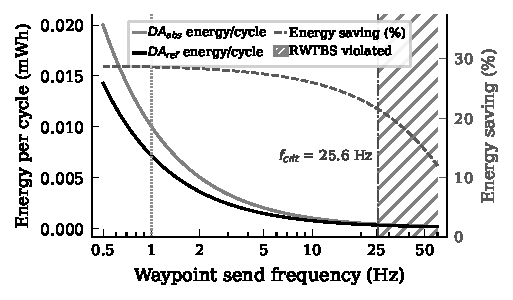
\includegraphics[width=\textwidth]{../energy_sensitivity.pdf}
\caption{Energy per cycle (left axis) and energy saving percentage (right axis)
  as a function of waypoint send frequency.  The light-red region marks the
  invalid operating regime where \RWTBS{} no longer holds.  The case study
  operating point is annotated at~1\,Hz.}
\label{fig:energysensitivity}
\end{figure}

\Cref{fig:energysensitivity} shows how the energy saving varies with waypoint
send frequency.  At low frequencies the drone spends most of its time sleeping
between infrequent messages, and the gap between the $\DAabs$ idle baseline
(36\,mW) and the $\DAref$ sleep baseline (22\,mW) translates into a large net
saving.  At the case study operating point of~1\,Hz the saving is~28.6\%,
consistent with the single-window estimate of~28.2\% from~\cref{sec:energy}.
As frequency increases, duty-cycle wake events become more frequent and the
fraction of time spent in sleep shrinks; by the critical threshold of~25.6\,Hz
the saving has fallen to~21.8\%.

The operator therefore faces a trade-off between communication frequency and
energy saving, but the trade-off has a hard upper boundary.  Above the critical
frequency, the saving is not merely smaller---the optimisation is formally
unsafe and the contract $C = (A,\,G)$ can no longer be guaranteed.  It is
precisely \RWTBS{} that makes this boundary computable rather than empirically
discovered through testing.  By Theorem~3, contract satisfaction is preserved
if and only if the refinement relation holds; the sensitivity analysis
identifies exactly the operating conditions under which it does.  An operator
can therefore read off directly from~\cref{fig:energysensitivity}: at the
current dispatch rate of~1\,Hz the energy saving is~28.6\%, and the maximum
frequency at which that saving remains formally valid is~25.6\,Hz.

The sensitivity analysis demonstrates that \RWTBS{} provides not merely a
binary accept/reject verdict for a specific software update, but a
characterisation of the operating envelope within which an update remains safe.
This is qualitatively stronger than what classical timed bisimulation could
offer even if it accepted the update: classical bisimulation would accept or
reject at a single operating point, not characterise a range.  The sensitivity
analysis therefore illustrates the practical value of the multi-view framework
of \cref{sec:vev}: virtual execution views can be systematically explored
across parameter ranges, and \RWTBS{} provides the formal mechanism to
determine which parameter values yield valid refinements.

% ══════════════════════════════════════════════════════════════════════
\section{Discussion}
\label{sec:discussion}

This case study demonstrates the semantic necessity of \RWTBS{}, beyond its
computational efficiency.  The synthetic and FMICS\,2021 benchmarks show that
Algorithm~1 scales to systems with hundreds of states and multiple clocks, but
they do not illustrate \emph{why} a relaxed bisimulation is needed.  The sugar
beet fleet example provides that illustration: a legitimate, energy-saving
software update that shifts input processing by up to 40\,ms is rejected by
classical weak timed bisimulation (which treats all observable timing shifts
equally) but accepted by \RWTBS{} (which distinguishes inputs from outputs).
The update preserves all output deadlines, satisfies the assume-guarantee
contract, and composes safely with the unchanged components---exactly the
guarantees a deployment engineer needs.

The role of the virtual execution view is central to this workflow.  The
duty-cycled drone agent was first prototyped in a ROS\,2 software-in-the-loop
environment, where its timing behaviour was observed and validated
experimentally.  The timed automaton $\DAref$ was then extracted from this
prototype as a formal model.  \RWTBS{} bridges the gap between the SiL
artefact (which exhibits the updated timing) and the deployment guarantee
(which requires that output deadlines and contracts are preserved).  Without
this bridge, the developer would need either a complete re-verification of the
parallel composition---potentially expensive for larger systems---or an informal
argument that the timing shift is ``small enough'' to be safe.

Several assumptions and limitations should be noted.  First, the model assumes
a FIFO buffer for incoming waypoint messages, with at most one pending message
at any time.  If multiple messages could be queued, the duty-cycle delay would
compound and the relaxation bound would need to account for queue depth.
Second, the alternating send/receive constraint (the drone processes one
waypoint per monitoring cycle) simplifies the interaction pattern.  A
concurrent multi-message protocol would require extending the model with
additional clocks and synchronisation.  Third, the 40\,ms duty cycle is
well within the 500\,ms end-to-end deadline budget: the report is sent at
55\,ms (11\%\ of the deadline) in the worst case, leaving 445\,ms for the FC
pipeline and treatment issuance.  If the duty cycle were increased to, say,
200\,ms, the report time would rise to 215\,ms (43\%\ of the budget), and the
FC pipeline budget would shrink to 285\,ms---potentially insufficient depending
on the FC's processing requirements.  In such a scenario, the \RWTBS{} checker
would correctly reject the update, as the output deadline margin would be
consumed.

\end{document}
